\chapter{Building Your Network Marketing Business}

This chapter follows Jim Rohn's original third talk as it appears in the curated LazyingArt LLC sequence, written from the Video2Book transcript and not from any validated board record. No mathematical screenshots survived review for this lecture, so every formula and diagram here is a cautious transcript-based reconstruction. The lecture nevertheless has a clear mathematical backbone, and we do best by following its order: philosophy first, then the hierarchy of profits over wages, then the arithmetic of part-time fortune, then the control split between wind and sail, then the law of averages, then the sower's distribution of outcomes, and only after that the catalog of skills and the broader architecture of a good life.

\section{From Farm Labor to Philosophy}

We begin where he begins: with an Idaho farm boy who knew how to milk cows and not much else. The opening is autobiographical, but it is not merely autobiographical. Rohn is establishing a baseline of low leverage. If a life can turn from there, then the cause of the turn becomes the real subject of the lecture.

That cause, in his own ordering, is not product first and not technique first. He says the opportunity changed his life, but only together with the philosophy that made the opportunity work. This is the hidden variable for the whole chapter. One may possess the best product, the finest support, and every useful technique, but without the driving philosophy nothing holds.

The lecture even pauses to explain why he wants notes taken. He recalls people returning years later with notebooks that shaped both business life and personal life. So the chapter is not only about earning. It is about portable sentences, repeatable distinctions, and a framework that can travel forward in time.

He briefly folds nutrition into the opening argument. That material is not part of the chapter's mathematical spine, but it matters structurally. It shows what he means by philosophy. Philosophy is not an opinion that floats above practice. It is belief turned into repeated study, repeated action, and repeated transmission.

\subsection{Question \& Answer}

\paragraph{Question.} Why is philosophy treated as more decisive than product or technique?

\paragraph{Answer.} Because product and technique are presented as available instruments, while philosophy governs whether we use them long enough, interpret setbacks correctly, and persist through the early discouragements. In the lecture's own hierarchy, philosophy is the active cause and technique is its means.

\section{Profits, Wages, and the Arithmetic of Part-Time Fortune}

Now the first explicit economic philosophy arrives, and he announces it exactly as a maxim: profits are better than wages. We can compress the spoken contrast into the shorthand
\begin{equation}
P > W,
\end{equation}
where \(P\) denotes profits and \(W\) denotes wages. This is editorial notation, not his own, but it captures the hierarchy he keeps repeating. He immediately supplies the phrase that goes with it:
\begin{equation}
W \longmapsto \text{a living},
\qquad
P \longmapsto \text{a fortune}.
\end{equation}
The lecture wants us to hear the contrast economically. Wages are not despised; they are simply bounded. They solve maintenance. Profits open an asymmetry.

He dramatizes the point politically. In Moscow he teaches capitalism not as oppression but as distributed ingenuity. Capital belongs in the hands of people, where imagination and enterprise live. The small-scale image is memorable: two bicycles, one to ride and one to rent. The large-scale image is East Germany:
\begin{equation}
\$1\text{ trillion}
=
\$500\text{ billion already spent}
+
\$500\text{ billion still to go}.
\end{equation}
The number matters because it makes philosophy material. A destructive doctrine is not merely false in a seminar room. It leaves a bill.

Only after the profit--wage hierarchy is firmly in place does he answer the practical question: how does an ordinary worker enter the world of profits? His answer is not heroic abandonment of the job. It is the magic of part-time. The initial commitment is deliberately modest:
\begin{equation}
h_{\mathrm{pt}} \in \{10,12,15\}\ \text{hours per week}.
\end{equation}
The transcript briefly garbles one line as ``four-day job,'' but the surrounding repetitions make the intended sentence plain: full-time on the job, part-time on the fortune. That is the first emotional shift. One is no longer only making a living; one has begun to work on fortune.

The lecture then gives us two milestones, and it is worth preserving them as a ladder:
\begin{equation}
P_{\mathrm{pt}} = W_{\mathrm{ft}},
\end{equation}
followed by
\begin{equation}
P_{\mathrm{pt}} = 2W_{\mathrm{ft}}.
\end{equation}
These are again editorial equalities, but they faithfully summarize the spoken sequence. First the part-time profit equals the full-time wage. Then it doubles it. Rohn says he reached the first threshold in less than six months, the second in less than a year.

\begin{figure}[t]
\centering
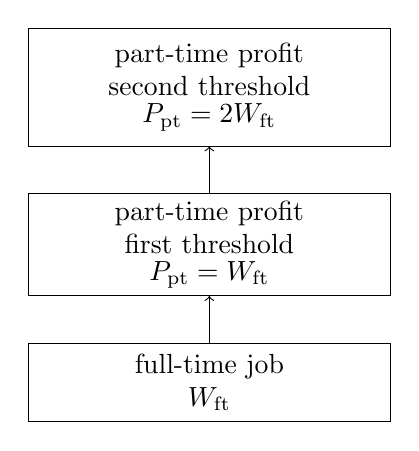
\begin{tikzpicture}[x=1cm,y=1cm]
\draw (0,0) rectangle (4.6,1.0);
\node at (2.3,0.5) {\shortstack{full-time job\\$W_{\mathrm{ft}}$}};

\draw (0,1.6) rectangle (4.6,2.9);
\node at (2.3,2.25) {\shortstack{part-time profit\\first threshold\\$P_{\mathrm{pt}}=W_{\mathrm{ft}}$}};

\draw (0,3.5) rectangle (4.6,5.0);
\node at (2.3,4.25) {\shortstack{part-time profit\\second threshold\\$P_{\mathrm{pt}}=2W_{\mathrm{ft}}$}};

\draw[->] (2.3,1.0) -- (2.3,1.6);
\draw[->] (2.3,2.9) -- (2.3,3.5);
\end{tikzpicture}
\end{figure}

What matters is not only the arithmetic. It is the invitation that the arithmetic creates. At the first threshold he can say: I found a way, part-time, to make as much as I make full-time. At the second threshold the invitation strengthens further: I found a way, part-time, to make twice what I make full-time. He even says that he delayed quitting the full-time job longer than was rational because he did not want to lose this electrifying recruiting story.

That explains the famous thousand-dollars-a-month comparison:
\begin{align}
\$1000/\text{month}_{\mathrm{ft}} &\Rightarrow \text{maintenance of an existing life},\\
\$1000/\text{month}_{\mathrm{pt}} &\Rightarrow \text{visible change in lifestyle}.
\end{align}
The money is not the whole story. It is what the money does. A part-time increment that produces vacations, cars, clothes, or visible breathing room makes strangers ask the right question: what are you doing?

\subsection{Question \& Answer}

\paragraph{Question.} Why is part-time profit more powerful as an invitation than the same amount earned full-time?

\paragraph{Answer.} Because the lecture treats part-time earnings as proof of a second mechanism. The same nominal amount is more persuasive when it alters lifestyle at the margin and leaves the original job still standing. The arithmetic is the same; the structure of the story is different.

\section{Wind, Sail, and the Logic of Self-Change}

Only after the part-time arithmetic has been stabilized does the lecture widen into a general law. It is not what happens that determines the future; it is what we do about what happens. Rohn gives us the sailboat image, and if we compress that image into a single schematic relation we may write
\begin{equation}
O = f(E,S),
\end{equation}
where \(E\) is the shared environment, \(S\) is the set of the sail, and \(O\) is the outcome. This is not formal economics or physics. It is a compact way of keeping his spoken distinction visible on the page.

The important part of the model is that the environment is broadly shared. The same wind blows on us all: the wind of disaster, opportunity, change, upside-down conditions, favorable conditions, unfavorable conditions, and, in his more social language, the economic, social, and political wind. So the difference in arrival after one year, three years, or five years cannot be assigned to wind alone.

He keeps reinforcing the point by a chain of regular recurrences:
\begin{align}
\text{fall} &\to \text{winter},\\
\text{day} &\to \text{night},\\
\text{expansion} &\to \text{recession},\\
\text{recession} &\to \text{expansion}.
\end{align}
And then he gives the widest compression of all:
\begin{equation}
\text{history} \approx \text{opportunity mixed with difficulty}.
\end{equation}
That approximation sign is ours, but the sentence is his. It is his way of saying that the mix changes in appearance, not in kind. Sometimes opportunity seems to dominate; sometimes difficulty seems to dominate. But the mixture remains.

He then returns to autobiography to make the law concrete:
\begin{equation}
\text{Years }1\!-\!6:\text{ broke},
\qquad
\text{Years }7\!-\!12:\text{ rich}.
\end{equation}
The lecture is explicit here. The second interval was not created by a political rescue. It was created by a change in philosophy: correcting the errors of the past and taking on new disciplines for the future. That is what a better sail means.

\subsection{Question \& Answer}

\paragraph{Question.} If the same wind blows on everyone, what exactly is under our control?

\paragraph{Answer.} Not the season, not recession itself, not the mere existence of difficulty. What is under our control is response: the interpretation, the discipline, the preparation, and the quality of action. That is why the sail, not the wind, becomes the operative variable.

From here the lecture makes its next turn with complete logic: for things to change, we have to change. The line is often quoted by itself, but in this talk it is the conclusion of the wind-and-sail picture. Once that is established, the later commands follow naturally. Do not wish it were easier; wish you were better. Do not wish for less problems; wish for more skills. Do not wish for less challenge; wish for more wisdom. The environment is not promised to us in gentle form. The task is to become the sort of person who can work within its actual form.

\section{Law of Averages, Scale, and Skill}

Now we arrive at the most sustained mathematical movement in the lecture. Rohn names the law of averages and treats it as a liberation from emotional chaos. If we do something often enough, a ratio will appear. We can introduce the cautious shorthand
\begin{equation}
r = \frac{s}{n},
\end{equation}
where \(n\) is the number of attempts and \(s\) the number of successes. He never states the formula this way, but the lecture's whole arithmetic is built from this relation.

The first case is deliberately plain:
\begin{equation}
10 \to 1.
\end{equation}
Talk to ten people, one says yes. That is the beginning of the ratio. The crucial addition is that once the ratio starts, it tends to continue. The lecture does not mean that the universe has signed a theorem in our favor. It means that repeated action produces a workable pattern.

\paragraph{Worked example.} If the current working ratio is one in ten, then the lecture urges us to think operationally rather than emotionally:
\begin{enumerate}
\item after \(10\) conversations, we expect roughly \(1\) success;
\item after \(20\) conversations, the same working ratio suggests roughly \(2\) successes;
\item after \(30\) conversations, roughly \(3\) successes.
\end{enumerate}
The point is not statistical exactitude. The point is that refusals become countable residue instead of personal drama.

The second move is even more important. Volume can beat efficiency. One person may convert at a dazzling rate; another, newly arrived, may convert poorly. But the larger count can still win:
\begin{align}
10 &\to 9,\\
100 &\to 10,
\end{align}
and therefore
\begin{equation}
10 > 9.
\end{equation}
This is the mathematical content behind the line, ``I make up in numbers what I lack in skill.'' The newcomer is not asked to envy the veteran. He is asked to compensate by count.

\begin{figure}[t]
\centering
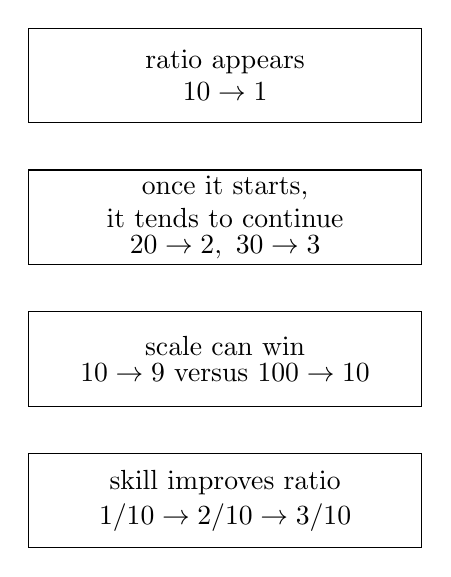
\begin{tikzpicture}[x=1cm,y=1cm]
\draw (0,4.8) rectangle (5.0,6.0);
\node at (2.5,5.4) {\shortstack{ratio appears\\$10 \to 1$}};

\draw (0,3.0) rectangle (5.0,4.2);
\node at (2.5,3.6) {\shortstack{once it starts,\\it tends to continue\\$20 \to 2,\ 30 \to 3$}};

\draw (0,1.2) rectangle (5.0,2.4);
\node at (2.5,1.8) {\shortstack{scale can win\\$10 \to 9$ versus $100 \to 10$}};

\draw (0,-0.6) rectangle (5.0,0.6);
\node at (2.5,0.0) {\shortstack{skill improves ratio\\$1/10 \to 2/10 \to 3/10$}};
\end{tikzpicture}
\end{figure}

The third move is that the ratio itself can improve. At first we may be at one in ten. Then, after enough repetition, we get two in ten. Later perhaps three in ten:
\begin{equation}
\frac{1}{10}\ \to\ \frac{2}{10}\ \to\ \frac{3}{10}.
\end{equation}
This is how the lecture connects discipline to skill. Action does not merely reveal the ratio; it changes the ratio.

He then normalizes failure with the baseball analogy:
\begin{equation}
\text{batting average}=.300
\qquad\Longrightarrow\qquad
\text{outs}=\frac{7}{10}.
\end{equation}
A .300 hitter fails seven times out of ten and is still elite. So the maxim follows: one does not have to bat \(1.000\) to make big money. One out of ten is fine. Two out of ten is terrific. Three out of ten is fabulous.

That is why the recruiting arithmetic is so calm:
\begin{equation}
10 \to 3\ \text{joiners} + 7\ \text{non-joiners}.
\end{equation}
The seven are not a disaster. They are the expected residue around the three. This is what makes the invitation script mathematically interesting. ``Come and be one of the seven'' is not defeatism. It is a way of protecting persistence from overinvestment in each single case.

\subsection{Question \& Answer}

\paragraph{Question.} How can someone with a worse ratio still outperform someone with a better one?

\paragraph{Answer.} Because the lecture compares total outcomes, not elegance in isolation. A person with \(9/10\) who speaks to only ten people gets nine results. A person with \(1/10\) who speaks to one hundred people gets ten. The weaker ratio loses in efficiency and wins in count.

\section{The Sower: Birds, Rocky Ground, Thorns, and Good Ground}

The lecture now deepens the law of averages by placing it inside a story. This is not a digression from the arithmetic. It is the arithmetic translated into a drama of categories. Rohn calls it the law of sowing and reaping, and he immediately says that the story of the sower contains the law of averages within it.

Two conditions are given at the beginning: the sower is ambitious, and the seed is excellent. That matters. We are not dealing with bad material. The later losses cannot be blamed on a lazy sower or worthless seed. The story begins with good inputs and still produces a distribution of outcomes.

\begin{figure}[t]
\centering
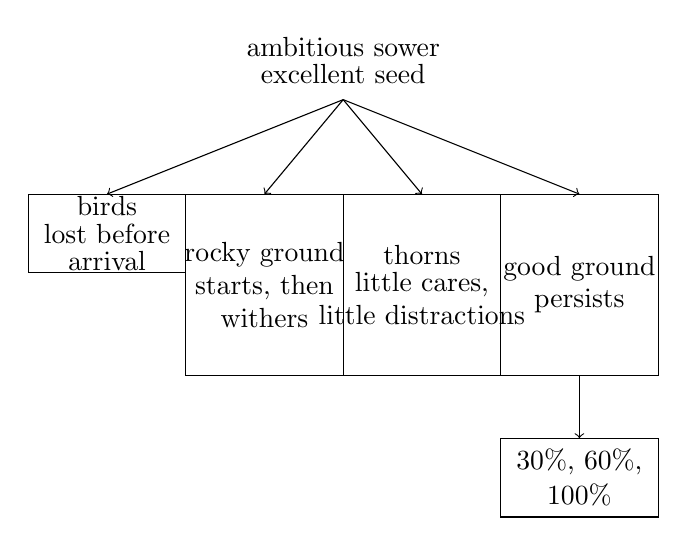
\begin{tikzpicture}[x=1cm,y=1cm]
\node at (0,6.0) {\shortstack{ambitious sower\\excellent seed}};
\draw[->] (0,5.5) -- (-3.0,4.3);
\draw[->] (0,5.5) -- (-1.0,4.3);
\draw[->] (0,5.5) -- (1.0,4.3);
\draw[->] (0,5.5) -- (3.0,4.3);

\draw (-4.0,3.3) rectangle (-2.0,4.3);
\node at (-3.0,3.8) {\shortstack{birds\\lost before\\arrival}};

\draw (-2.0,2.0) rectangle (0.0,4.3);
\node at (-1.0,3.15) {\shortstack{rocky ground\\starts, then\\withers}};

\draw (0.0,2.0) rectangle (2.0,4.3);
\node at (1.0,3.15) {\shortstack{thorns\\little cares,\\little distractions}};

\draw (2.0,2.0) rectangle (4.0,4.3);
\node at (3.0,3.15) {\shortstack{good ground\\persists}};

\draw[->] (3.0,2.0) -- (3.0,1.2);
\draw (2.0,0.2) rectangle (4.0,1.2);
\node at (3.0,0.7) {\shortstack{$30\%$, $60\%$,\\$100\%$}};
\end{tikzpicture}
\end{figure}

First come the birds. In operational language, these are the people who were going to come to the meeting and then do not appear. The idea was stolen. The prospect is gone before engagement even begins. Here the lecture gives a practical command: do not chase birds. If we chase birds, we leave the field. The right response is not investigation without end. It is the small stabilizing phrase, ``Isn't that interesting?'' and then continued sowing.

Second comes rocky ground. Here the seed begins to grow. A person starts, shows life, and then withers under the first heat. Rohn's short line is exact: some do not stay. Again the lecture refuses the permanent enrollment in the ``why'' class. These are categories, not metaphysical puzzles.

Third come the thorns. These are not grand disasters. They are little cares, little distractions, screen doors off the hinges, trash in the garage, small maintenance claims that choke larger opportunity. That detail is one of the chapter's best operational observations. Big opportunities are often not defeated by gigantic enemies. They are defeated by the cumulative authority of little things.

At this point the lecture gives one of its strongest practical lines:
\begin{equation}
\text{sow}
\longrightarrow
\text{loss}
\longrightarrow
\text{discipline disappointment}
\longrightarrow
\text{sow again}.
\end{equation}
Disciplining disappointment is not decorative advice here. It is the condition of remaining in the field long enough for the law of averages to turn in our favor.

\subsection{Question \& Answer}

\paragraph{Question.} What do we do when people disappear, get distracted, or refuse to persist?

\paragraph{Answer.} We classify rather than dramatize. Some are birds, some are rocky ground, some are thorns. We do not chase every loss, and we do not stop sowing. The lecture's answer is procedural: accept the category, discipline disappointment, and continue.

Now the good news arrives. Good ground exists, and if the sowing continues the seed will eventually land there. But even good ground is not uniform:
\begin{equation}
Y \in \{30\%,60\%,100\%\}.
\end{equation}
The outputs differ. Some produce thirty, some sixty, some a hundred. Rohn again refuses to turn this into an endless inquiry. Why does one person do thirty and another a hundred? That, too, is a class he declines to spend his life explaining. The practical instruction is narrower and better: let the thirties do thirty, let the sixties do sixty, let the hundreds do a hundred. Do not try to force a false uniformity onto the field.

\section{Skills, Recruiting, and Service to the Many}

Only after the discipline of process has been built does the lecture open its long list of skills. This order matters. Technique is not the hidden cause; it is the flowering of the earlier philosophy. Still, once the philosophy is secure, skill matters enormously.

The first skill is sales, though he softens the word into sharing. In his description, one uses the product, gathers testimony, explains its merits, and invites participation. The numerical claim is blunt:
\begin{equation}
I_{\text{after sales}} \approx 5\,I_{\text{before sales}}.
\end{equation}
He says sales multiplied his income by five. The exact baseline is modest, but the multiplier is the point. Skill changes scale.

The next skill is recruiting, and the lecture handles it relationally. Recruiting includes invitation, presentation, and follow-up. A sponsor is not merely a closer; a sponsor is mother and father to a new life. He nourishes it and protects it. He is also a bridge: from darkness to light, from skepticism to faith, from not knowing to knowing, from low confidence to growing confidence. That metaphor matters because it tells us what recruiting is supposed to feel like on the page: stewardship rather than extraction.

Then come organizing and promotion. Organizing is getting people to work together, which he calls magic precisely because it is difficult. Promotion is smaller-scale ingenuity: recognizing small steps, creating local categories, rewarding progress before the company-level banners arrive. He is mathematically suggestive even here. Working together is valuable because it produces shared testimonials, shared momentum, and therefore multiplication rather than simple addition. As a maxim, not as a theorem, the lecture compresses the point into the biblical line that if two or three agree on a common purpose, nothing is impossible.

Communication follows. He even sketches a simple meeting logic: identification, reason, obstacle, confession, solution. But the real lesson is more basic: he did it again. The first presentation was awkward; then he did it again. The first step away from the podium was uncomfortable; then he did it again. Communication becomes a skill by repetition in public, not by waiting to feel ready in private.

Training and teaching come next. Training is how the business works. Teaching is how life works. And then comes the final skill in the sequence: inspiration, which he defines as helping people see themselves a little higher than they presently stand, and helping them believe that the higher picture is reachable.

Only now does the lecture widen to greatness and service. The formula is repeated through several voices, but the core line is stable:
\begin{equation}
\text{service to many} \longrightarrow \text{greatness}.
\end{equation}
And in Ziglar's sharper version:
\begin{equation}
\text{help enough people get what they want}
\Longrightarrow
\text{you can have what you want}.
\end{equation}
The arithmetic implied here is not formal, but it is clear. If our activity affects only a few lives, it earns at one scale. If it affects dozens, hundreds, or thousands, it earns at another. The business becomes a device for scaling service.

\subsection{Question \& Answer}

\paragraph{Question.} How does serving more people become a mathematically scalable route to wealth and influence?

\paragraph{Answer.} Because the lecture treats recruiting, organizing, and sponsoring as multiplicative mechanisms. One does not merely transact with one more person. One helps establish people who themselves begin to influence others. That is why the scale moves from a few, to many, to dozens, hundreds, and thousands.

\section{Deserve, 80/20, Capital, and the Good Life}

The lecture now narrows again, from greatness to sponsor discipline. We are told to work with the people who deserve it, not simply the people who need it. The grounding is agricultural. The harvest is linked to planting, not to wanting:
\begin{equation}
\text{if you plant, you reap}
\qquad\text{not}\qquad
\text{if you need, you reap}.
\end{equation}
That is why he says we must respond like life itself, to deserve rather than to need.

The local sponsor rule becomes an update law:
\begin{align}
\text{you step} &\Rightarrow \text{I step},\\
\text{you respond} &\Rightarrow \text{I respond},\\
\text{you try} &\Rightarrow \text{I try},\\
\text{you do not step} &\Rightarrow \text{I do not step}.
\end{align}
This is one of the clearest operational blocks in the lecture. Attention follows movement. Help follows action. Sympathy does not disappear, but it is no longer confused with structure.

Then comes the 80/20 allocation:
\begin{align}
80\% &\text{ of the people do }20\%\text{ of the business},\\
20\% &\text{ can therefore be handled individually},\\
80\% &\text{ must largely be handled by group work}.
\end{align}
The point is not contempt for the eighty percent. Group work is said to be powerful and less confrontational. The point is simply that attention is finite and must be organized.

The same realism sharpens the next line: one may help a thousand, but one cannot carry three on one's back. Help scales; carrying does not. That is why he adds the pear-tree image. One cannot hang apples on a pear tree and expect a changed harvest. One cannot change people directly; people can change themselves. This is not cynicism. It is another boundary condition.

Capital is then demoted below skill:
\begin{equation}
\text{money without skill} \not\Rightarrow \text{future},
\qquad
\text{skill} \Rightarrow \text{future}.
\end{equation}
He says plainly that it is not money that buys the future; it is skill. Money without courage remains poor. Money without ambition remains stalled. A dollar and some ambition may be enough. That is the setting in which his late, noisy capitalism formulation makes sense:
\begin{equation}
\text{buy}\to\text{sell}
\qquad\text{or}\qquad
\text{sell}\to\text{buy}.
\end{equation}
The wording is garbled in the transcript, so we keep the notation minimal. But the operational claim is clear enough: entry into enterprise does not always require waiting for large initial capital; ingenuity and motion can reverse the order.

Now the lecture broadens one last time. The greatest value in life is not the bank account but living a good life. He gives us a short list: productivity, good friends, spirituality, study--practice--teach, and the refusal to miss what nourishes the soul. The music and quotation material belongs here. It is not part of the numerical spine, but it explains why the final economic principle is not purely economic:
\begin{equation}
\text{live well} \Longrightarrow \text{earn well}.
\end{equation}
The lecture does not mean that refinement automatically mints money. It means that a nourished inner life changes the texture of the voice, the face, and the personality, and therefore changes the human instrument that conducts all the earlier business skills.

The inner circle is the final form of this idea. One's closest people are not external decoration. They are a power source. If we nourish them, they nourish us. And from there the lecture ends on its deepest motive: participation in the miracle process. Changing a life, rescuing someone from oblivion, building an organization worthy of testimony, and sending notes forward into someone else's future. The final image is beautiful and exact: he goes with the audience in their notes, and they go with him in his thoughts and in their eventual testimonial.

\section{Summary}

The chapter unfolds in a strict order. First comes philosophy, because without it nothing else works for long. Then comes the first economic distinction, \(P>W\), together with the part-time ladder \(P_{\mathrm{pt}}=W_{\mathrm{ft}}\) and \(P_{\mathrm{pt}}=2W_{\mathrm{ft}}\). Then the lecture widens from money to control: the same wind blows on everyone, but the sail can be set differently. From there we pass to self-change, and then to the law of averages, where action becomes countable and persistence becomes rational. The sower story then converts ratio into drama: birds, rocky ground, thorns, good ground, and the discipline of disappointment. Only after that foundation does Rohn give the skill list: sales, recruiting, organizing, promotion, communication, training, teaching, inspiring. The final movement says that service scales, attention must be earned, skill matters more than capital, and business success finally sits inside a larger task, which is to live well enough that one's work carries force.